%*******************************************
\section{App Evaluation}
%*******************************************
\label{s:evaluation}
After having designed and implemented the app, the evaluation of our work remains as a final step. This chapter describes our evaluation process.
 The app will be evaluated with the aid of a user study.
 After introducing our study design, we will state our hypotheses and explain how we are going to measure our statements.
 Finally, we will analyze our results and state our conclusion.


%===========================================
\subsection{Participant Recruitment}
%===========================================
\label{s:participant_recruitment}
This section deals with the participant recruitment for the user study.
As an incentive to attend our user study a gift card was raffled among 4 users.
A major challenge was not to address close friends in order to receive unbiased and honest feedback. 
To reach potential participants we proceeded as follows:

\begin{description}[leftmargin=0cm]
\item[Flyer:]  We prepared a flyer with the most important information. 
In this flyer we told the user that a learning app about Internet security in general will be tested. 
We did not mention the specific topic of phishing in advance because we did not want potential participants to read up about it before the study.
Copies of this flyer were hung on blackboards of student dorms and some other buildings at the university.
\item[E-Mail to Professors:] We additionally distributed the flyer to a number of professors in our university and asked them to forward it to their students and/or teaching staff.
We did not forward the flyer to computer science professors or professors of similar technical majors since their students and staff most likely do not match our target group.
\item[Online Social Networks:] We contacted our friends in online social networks and asked them to ask friends whether they would be willing to participate in our user study.
Additionally, we posted the flyer in university groups of online social networks with the hope some people might be interested in participating.
\item[Further Networks:] Finally, we called friends we could not reach via online social networks and asked them if they knew anybody who would participate.
\end{description}
In \autoref{s:participant_recruitment_texts} copies of our e-mails to the professors and of our flyer can be consulted.
Note that we had to split the user study into groups of 4 participants due to the lack of available smartphones.
Moreover, our flyer originally said that the best participant of each group would win the gift certificate.
However, we recognized that the winning chance might not be equal for every participant due to varying expertise, for example, or other possible technical problems such as app crashes.
For this reason we asked the participants at the beginnig of each study whether they agreed to raffle the gift certificate instead.
To express our appreciation to each participant we decided to offer cookies and other kinds of sweets.
Additionally, the participant who performed best was awarded with a ``Golden Anti-Phish Certificate'', all other participants received a ``Silver Anti-Phish Certificate'' (cf. \autoref{s:antiphish_certs}).

%===========================================
\subsection{Study Design}
%===========================================
For our user study we chose a within-subject design, i.e. a ``before and after app'' study with the same group of people.
The advantages of this design can be summarized as follows:
Within-subject deals better with variability associated with individual differences compared to between-group design, where different groups would be considered who do and do not play the app.
A major drawback of the within-subject design, however, is the learning effect.
We are not able to clearly distinguish whether a behavior change after playing the app is a result of the app intervention or of learning effects.
Yet, our results showed that the learning effects seemed to have only a minor impact (cf. \autoref{s:hypanalysis}).

\autoref{fig:study_structure} illustrates the structure and process of our study. In the following, we dwell on each of the consecutive steps:
\begin{enumerate}
	\item \textit{Informed Consent:} Before starting the user study the participants have to sign an informed consent.
This form briefly explains what the study is about and clarifies that the participant is not obliged to finish the study.
If the user terminates the study before finishing it, however, he cannot participate in the gift certificate raffle.
Optionally, the user can agree with the anonymous publication of the:
	\begin{enumerate}
		\item transcriptions of the study (recordings will be deleted after the study)
		\item filled out surveys
	\end{enumerate}

	\item \textit{General-Survey Before:} At the beginning the participants have to fill out a general survey, where they have to judge their own knowledge on the topic of Internet security in general.
 For instance, they are asked whether it is easy for them to distinguish legitimate e-mails and websites from fake ones.

	\item \textit{Website-Survery Before:} In this part of the user study the participants get a list of screenshots of websites.
 The screenshots had been taken with the standard browser of an Android tablet.
 In total, the user is shown 16 screenshots, with 8 phishing and 8 valid URLs.
 The user has to decide whether he would enter confidential data on the shown website.
 Additionally, he has to encircle the part of the screenshot which was the primary reason for his decision.
 Then, the user has to indicate how sure he was about his answers on a Likert scale.
 Finally, the user is asked whether he knows the vendor of the website and whether he has an account there.
 The list of the used URLs can be found in \autoref{example_urls_before}.
Note that we used the same order for every participant's survey, i.e. everybody was confronted with these URLs in the same order.

	\item \textit{Play App:} Here, the users get the smartphones in order to play the app.
 To save time, we skipped the introduction 2 part (how to access the address bar) for the user study.
 The user has half an hour to play.
 Afterwards, they are asked to put the smartphones aside.
 Then, we collect the smartphones and note the reached points for each level.
Note that the selection of URLs in our app is randomized.
This means that the users were confronted with random and thus possibly different URLs.

	\item \textit{Website-Survery After:} After playing the app, the participants get a second website-survey.
 In this, all examples of the previous survey are included.
 Moreover, it contains 8 further website screenshots of which 4 represent phishing and the other 4 legitimate URLs.
  The list of the used URLs can be found in \autoref{example_urls_after}.
Note that we used the same order for every participant's survey, i.e. everybody was confronted with these URLs in the same order.

	\item \textit{General-Survey After:} Here, the participants are asked to complete a form with questions pertaining to their person, for example, their age or course of study.
 This form does also contain questions related to the System Usability Scale (SUS)~\cite{sus}, which is supposed to assess the usability of our app, and questions regarding the users' impression of the app.
	
	\item \textit{Certificates:} At this point the official part of the study is finished.
We thank the users for their participation and award a ``Golden Anti-Phish Certicate'' to the best participant of the current group.
All other attendants receieve a ``Silver Anti-Phish Certificate''.
Next, the gift certificate is raffled.

	\item \textit{Debriefing:} After the official end of the study (after handing out the certificates) we asked the participants if they were willing to stay for an optional debriefing, where they could ask questions or provide their remarks in person. In case a participant did not want to stay for this debriefing, he was free to go.
\end{enumerate}



\begin{figure}[hHtbp]
\centering
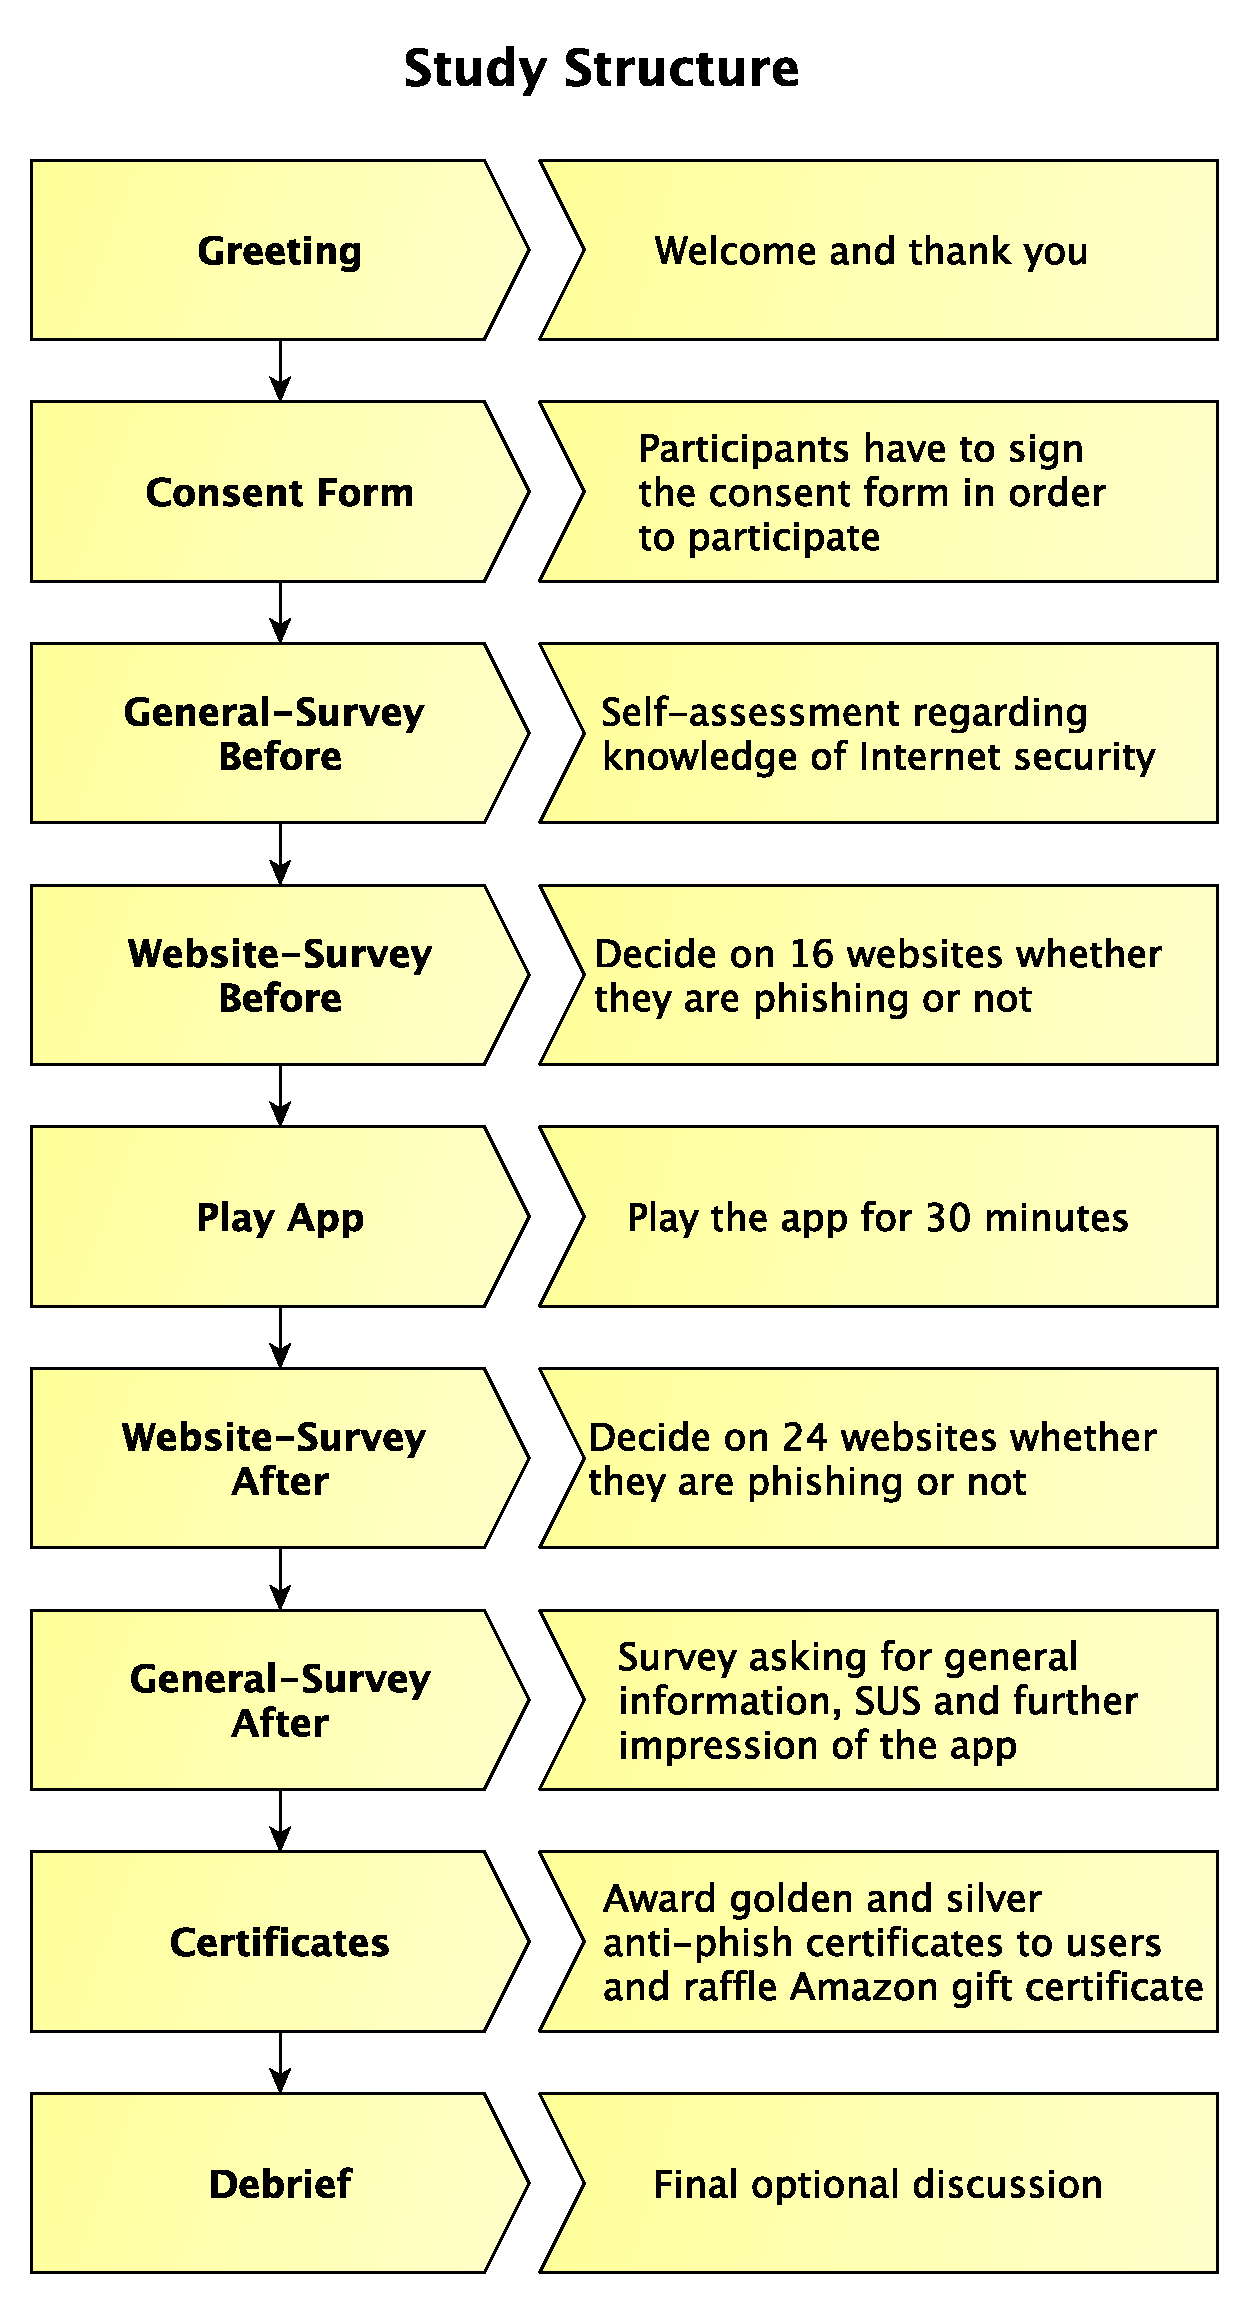
\includegraphics[height=0.9\textwidth]{study_structure.pdf}%
\caption{Structure and process of our final user study}%
\label{fig:study_structure}%
\end{figure}

%===========================================
\subsection{Hypotheses}
%===========================================
In order to evaluate the effectiveness and usability of our app we formulated the following hypotheses and measurements.

\begin{enumerate}
	\item \textit{Hypothesis 1 - Mistakes:} After playing the app, the users make significantly less mistakes when deciding whether a website is a phish or not than before using the app.\newline
	Measurement: Correctly identified websites in ``Website-Survery After'' (phish or no phish) $>>$ correctly identified websites in ``Website-Survery Before''
	\item \textit{Hypothesis 2 - URL Based Decision:} After playing the app, the users primarily base their decision whether a website is a phishing website or not significantly more often on the URL compared to before playing the app.\newline
	Measurement: Number of URL markings in ``Website-Survery After'' $>>$ number of URL markings in ``Website-Survery Before''
	\item \textit{Hypothesis 3 - URL Comprehension:} After playing the app the user understands that the domain of a URL is the most important criterion to detect phishing websites\newline
Measurement: Number of marked URL domains in ``Website-Survery After''  $>>$ number of marked URL domains in ``Website-Survery Before'' 
	\item \textit{Hypothesis 4 - Good Usability:} The usability of the app is above average. \newline
Measurement: A System Usability Scale (SUS) $>$ 68 can be considered above average usability~\cite{sus}.
\end{enumerate}

%===========================================
\subsection{Classifying Markings}
%===========================================
\label{s:markings}
One part of the study involved marking the area on a given website which contributed to the users' decision on whether they thought the website was fraudulent or legitimate.
In order to assess these markings, for the measurement of hypothesis 3, we needed to define respective codings.
To digitize the markings of the participants we proceeded as follows:
One of us read out the markings and the other wrote them down. Occasionally the writing person checked whether he had the same impression. When the reading person was uncertain he also asked the writer. In some very uncertain cases we consulted a third party.
Here, we provide an overview of the regions participants marked during the website-surveys and how we coded them internally for the evaluation.
Furtheremore, we discuss our marking interpretations and outline several interpretation problems, due to imprecise markings, and how we approached those.

%.........................................................................................................
\subsubsection{Marking Examples}
%.........................................................................................................
The following list summarizes the codings we used for the markings of the participants.

\begin{enumerate}
	\item\textit{None:} Occasionally, participants did not mark or encircle anything of the screenshot. In our raw data this is coded as none (cf.~\autoref{fig:m_none}).
	\begin{figure}[H]
				\centering
				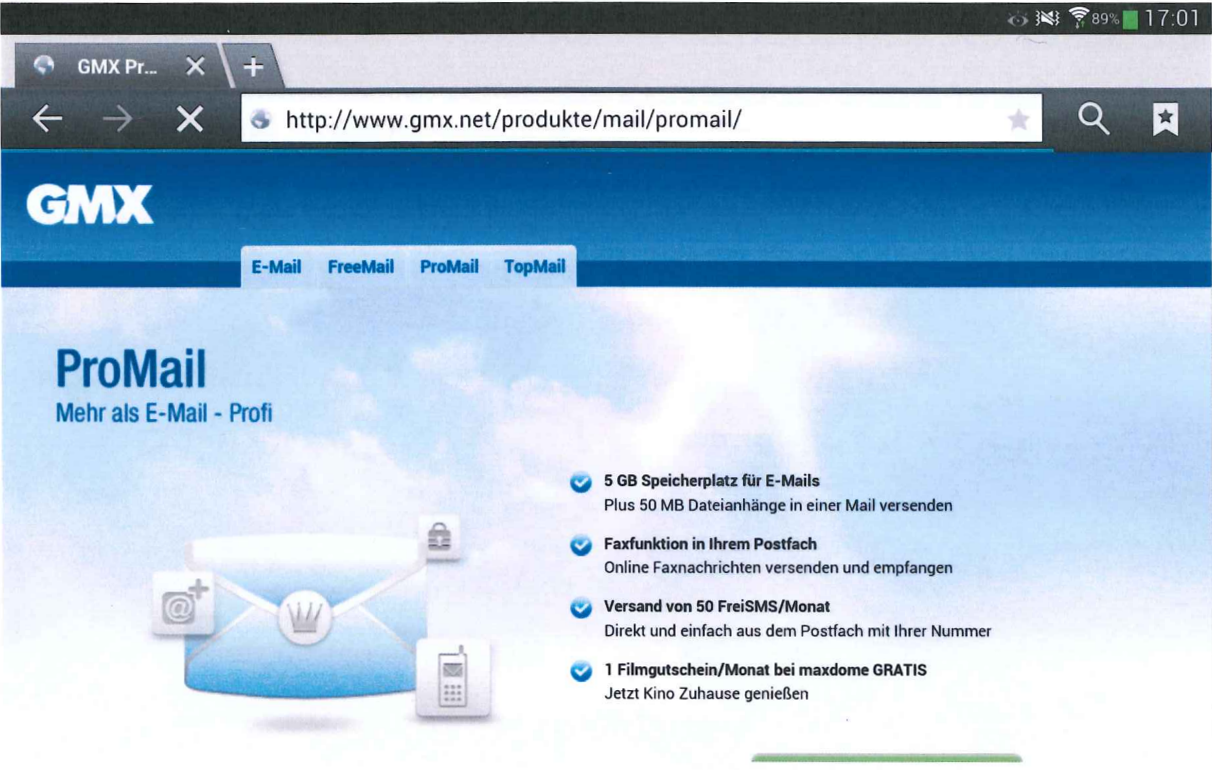
\includegraphics[width=0.8\textwidth]{m_none.png}
				\caption{Nothing marked}
				\label{fig:m_none}
				\end{figure}
	\item\textit{Favicon or Padlock:} The marking of a favicon or padlock is trivially coded accordingly (cf.~\autoref{fig:padlock}).
	\begin{figure}[H]
	\centering
	
\includegraphics[width=0.8\textwidth]{m_padlock.png}
	\caption{Padlock marked}
	\label{fig:padlock}
	\end{figure}
	\item\textit{Content:} If anything else than the URL itself, a part of the URL, a favicon, or a padlock is marked then this is coded as content (cf.~\autoref{fig:content}).
	\begin{figure}[H]
	\centering
	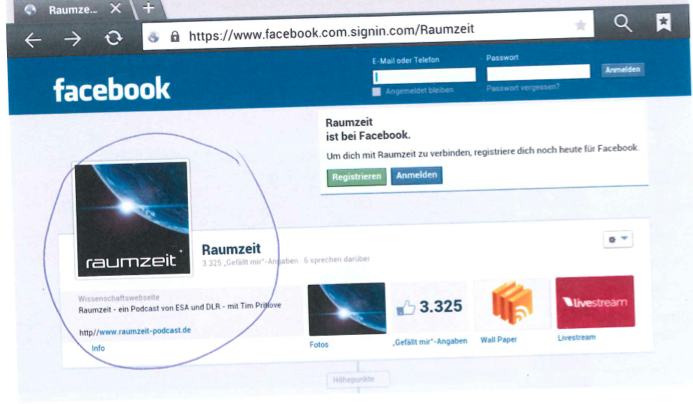
\includegraphics[width=0.8\textwidth]{m_content.png}
	\caption{Content marked}
	\label{fig:content}
	\end{figure}
	\item\textit{Scheme:} If the scheme or a part of the scheme in a URL is marked, this is coded as scheme (cf.~\autoref{fig:m_scheme}).
	\begin{figure}[H]
			\centering
			
\includegraphics[width=0.8\textwidth]{m_scheme.png}
			\caption{Scheme marked}
			\label{fig:m_scheme}
			\end{figure}
	\item\textit{Host:} Marking the host results in an according coding (cf.~\autoref{fig:m_host}).
		\begin{figure}[H]
		\centering
		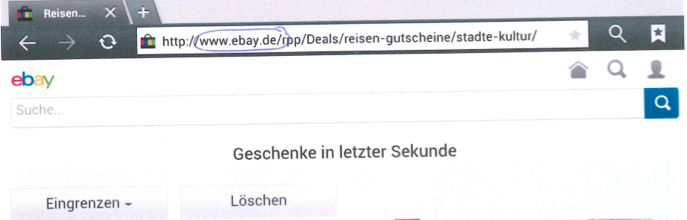
\includegraphics[width=0.8\textwidth]{m_host.png}
		\caption{Host marked}
		\label{fig:m_host}
		\end{figure}
	\item\textit{Domain:} In case a participant marks a domain (cf.~\autoref{fig:m_domain}) or the substring of a domain (cf.~\autoref{fig:m_domain_substring}) this is coded as domain or domain substring accordingly.
For the measurement of hypothesis 3, domain as well as domain substring markings are considered domains.
\begin{figure}[H]
\centering

\includegraphics[width=0.8\textwidth]{m_domain.png}
\caption{Domain marked}
\label{fig:m_domain}
\end{figure}
\begin{figure}[H]
\centering

\includegraphics[width=0.8\textwidth]{m_domain_substring.png}
\caption{Domain substring marked}
\label{fig:m_domain_substring}
\end{figure}

	\item\textit{URL:} All other markings are coded as URL and measured as such. For instance, the subdomain of a URL is coded as URL (cf.~\autoref{fig:m_url_02}).
	\begin{figure}[H]
	\centering
	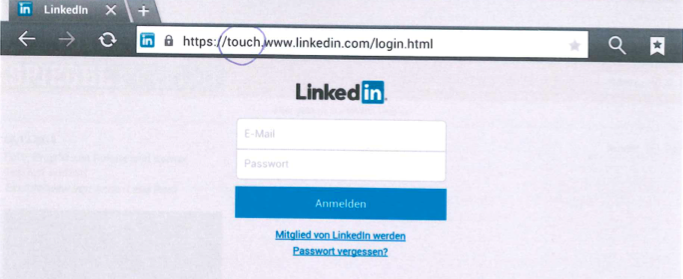
\includegraphics[width=0.8\textwidth]{m_url_02.png}
	\caption{Subdomain marked, coded as URL}
	\label{fig:m_url_02}
	\end{figure}
\end{enumerate}

%.........................................................................................................
\subsubsection{Interpretation Problems}
%.........................................................................................................
\label{s:intprobs}
While assessing and digitalizing our data we had to face some interpretation problems which we exemplify in the following.
In such cases we had no choice but striving to interpret the samples as objectively as possible.
\autoref{fig:m_content_or_host}, for instance, shows a marking where the circle includes the content (YouTube logo) as well as the host. 
For this sample, we decided to code the marking as host.
The next example in \autoref{fig:m_domain_or_not} shows a marking where a subdomain and the domain is marked. 
When we faced examples like this we decided to code it as domain in case a subdomain is only partially marked, so that there is an indication that the user just did not make his markings precise enough.
If the subdomain is obviously marked deliberately, i.e. clearly inside the circle, this kind of sample is coded as URL.
In this case we see that the subdomain is inside the circle and coded this sample as URL accordingly.
Another frequently occurring sample is one where two areas are marked, even though we explicitly asked to mark only one.
In these cases we decided as follows: in case a marking is obviously striking due to a thicker circle, for instance, the more emphasized area is chosen for coding.
In case both markings were equal, we joined the markings and decided based on that.
In \autoref{fig:m_url}, for instance, a participant marked the scheme and the host separately. 
We cannot observe any emphasis on one of the markings.
Therefore, we chose to code this sample as URL.
Finally, there were samples where the user correctly identified a phishing website.
However, instead of marking the domain as the reason (as it is done in the app), some users marked the attacked part instead.
\autoref{fig:m_attack_recognized} illustrates such an example.
In fact, marking the attacked part is justified. 
Yet, we had to code such samples as URL since there is no clearcut way of defining whether an attacked part of a URL was recognized or not.
In the contrary, the domain of a URL can always be considered as the attacked part. Therefore, users should primarily base their decisions on domains.

\begin{figure}[H]
\centering
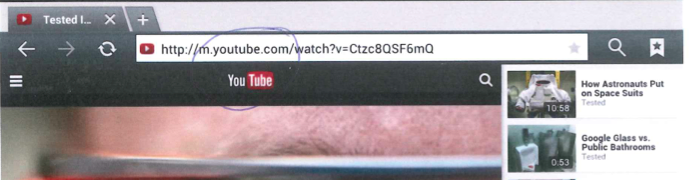
\includegraphics[width=0.8\textwidth]{m_content_or_host.png}
\caption{Host or content marked?}
\label{fig:m_content_or_host}
\end{figure}

\begin{figure}[H]
\centering
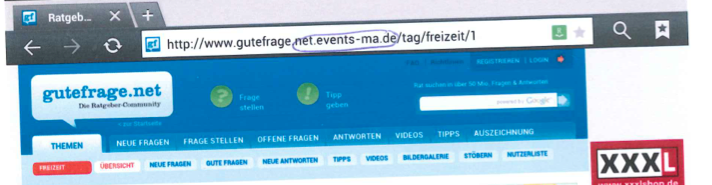
\includegraphics[width=0.8\textwidth]{m_domain_or_not.png}
\caption{Domain or URL marked?}
\label{fig:m_domain_or_not}
\end{figure}

\begin{figure}[H]
\centering

\includegraphics[width=0.8\textwidth]{m_url.png}
\caption{Scheme or host marked?}
\label{fig:m_url}
\end{figure}

\begin{figure}[H]
\centering

\includegraphics[width=0.8\textwidth]{m_attack_recognized.png}
\caption{Attack marked}
\label{fig:m_attack_recognized}
\end{figure}

%===========================================
\subsection{Results and Analysis}
%===========================================
This section presents our results and analyzes them. 
We start with discussing the representativeness of our participants and proceed with illustrating interpretation problems we faced while we assessed the website-surveys.
Therafter, we evaluate our hypotheses and proceed with further exploration of our results, followed by discussing the limitations of our study.
Finally, this chapter concludes with a disussion of our results and a corresponding summary. 
%.........................................................................................................
\subsubsection{Representativeness of Our Participants}
%.........................................................................................................
\label{s:representativeness}
In \autoref{s:target_group_def} we defined preconditions that users have to hold in order to match our target group.
We aspired to recruit participants who hold these preconditions as far as possible.
In the following we discuss the representativeness of our participants with the aid of these preconditions.

\begin{description}[leftmargin=0cm]
	\item[Attackability:] Generally, we took care that the people we recruited do not have extensive prior knowledge on this topic.
For example, our flyer asked for non-specialists.
Yet, we were not able to assure beforehand that we would only have non-specialist participants.
In such a case we had to rule them out for our analysis afterwards.
Unlike in our initial survey (cf. \autoref{s:survey}), we did not exclude electrical engineers or computer scientists in general from our final user study.
The problem with the phishing survey was that it did not give us enough indication whether a particular participant was too familiar with the topic.
Therefore, we had to imply that computer scientists and electrical engineers are too skilled, even if this does not necessarily need to be the case in reality.
In fact, there might be computer scientists or electrical engineers who can learn something from our app.
In contrast to the phishing survey, in our final user study we were able to determine a user's prior knowledge more precisely with the aid of the website-survey before.
Therefore, we did not primarily consider their course of study or field of work, but rather how well they performed in the website-survey before playing the app (cf. \autoref{s:hypanalysis}).
This way we assured that the considered participants were potential targets of phishing.
	\item[Android Users:] For the study we considered it important that our participants own a smartphone in general since we wanted the focus to be on our contents. This way, we minimize failures resulting from general operating difficulties.
Since we provided the required smartphones during the study we had no need to recruit participants who obligatorily own an Android smartphone.
Overall, 7 of 17 participants owned an Android and 10 of them owned an iOS smartphone, i.e. every attendant was a smartphone owner.
	\item[Language:] Participants of our study need to know German because all of the app texts are in German. This was ensured by providing flyers and e-mails in German language so that persons who do not master the German language do not feel to be addressed.
All of our participants could speak and read German.
\item[Motivation:] We mainly target users who download our app by choice and thus have a basic motivation to learn something from it.
For the user study our flyer was supposed to draw interested persons to participate in our study.
Furthermore, we created an additional incentive to attend our study by raffling a gift certificate.
\end{description}
Finally, we aspired to recruit participants who are not close friends of ours in order to minimize biases as far as possible.
%.........................................................................................................
\subsubsection{Analysis of Our Hypotheses}
%.........................................................................................................
\label{s:hypanalysis}
In total 19 participants attended our study.
As discussed in \autoref{s:representativeness} we did not exclude any participant beforehand because by means of the website-survey before we were able to precisely determine the prior knowledge of the participants.
Ultimately, we had to sort out two participants for the results and analyses of our study:

\begin{enumerate}
	\item\textit{Outlier:} \autoref{fig:outlier} depicts the performance of our participants.
	It illustrates how many URLs were correctly identified by how many users.
	Evidently, there is an outlier among our participants. 
	One user gave 15 correct answers to 16 questions.
	This means that he has too much prior knowledge on this topic and thus does not match our target audience.
	Therefore, this participant is not considered for our further elaborations.

\begin{figure}
\centering
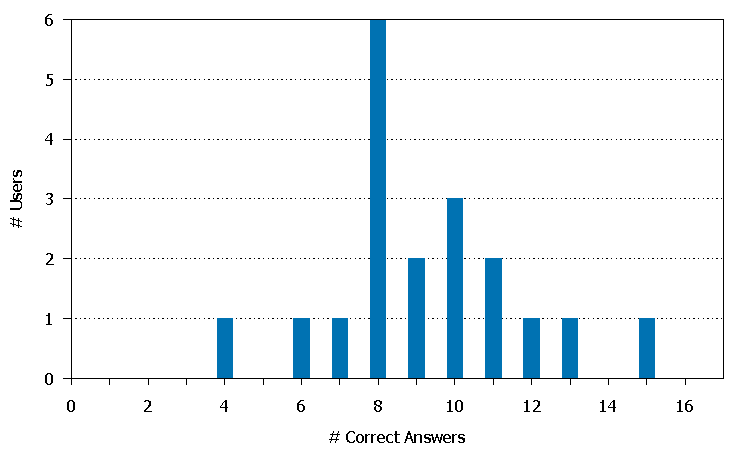
\includegraphics[width=0.7\textwidth]{outlier.pdf}
\caption{Performance of unfiltered users before playing the app depicting an outlier}
\label{fig:outlier}
\end{figure}

	\item\textit{Seriousness:} Another participant obviously did not engage himself to play our app.
	During the 30 minutes of playing the app the user managed to complete the awareness part and level 1 (identify domain) only.
	More importantly, we saw the user playing around with the smartphone instead.
	Since this user did not seem to take our study and app seriously we decided to sort him out for further considerations.
\end{enumerate}
In the following we present the results of our study corresponding to our hypotheses.

\begin{figure}
\centering
\subfigure[Before]{\label{fig:hyp1resultsbefore}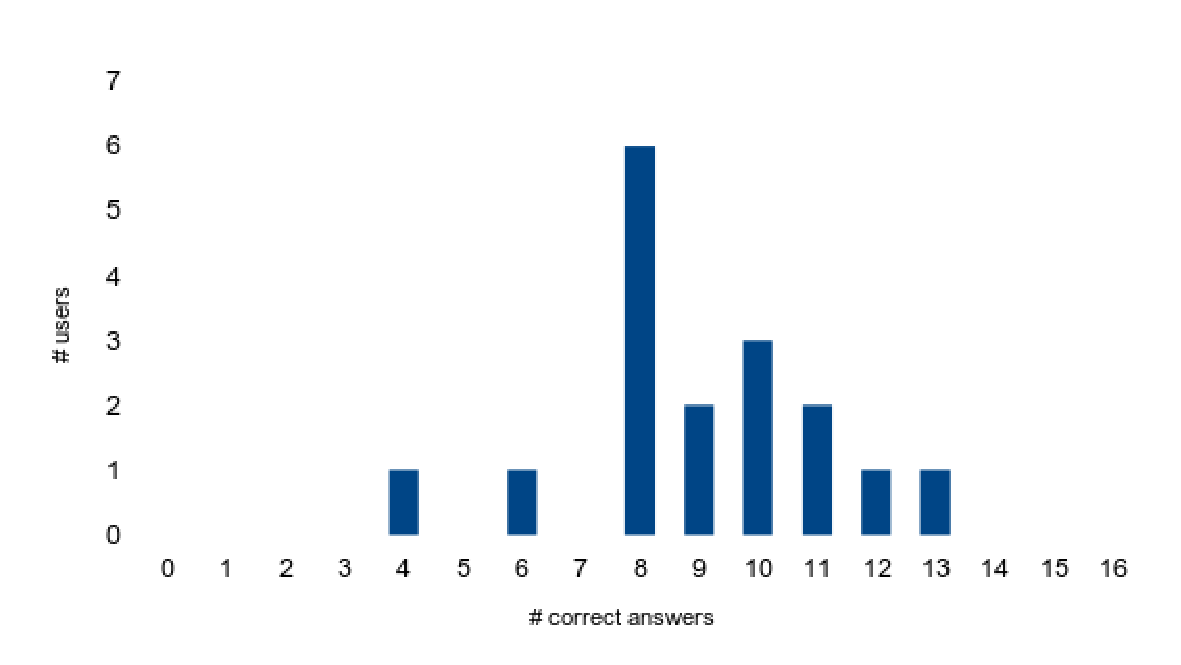
\includegraphics[width=0.45\textwidth]{hyp1b.pdf}}
\subfigure[After (Including All URLs)]{\label{fig:hyp1resultsaall}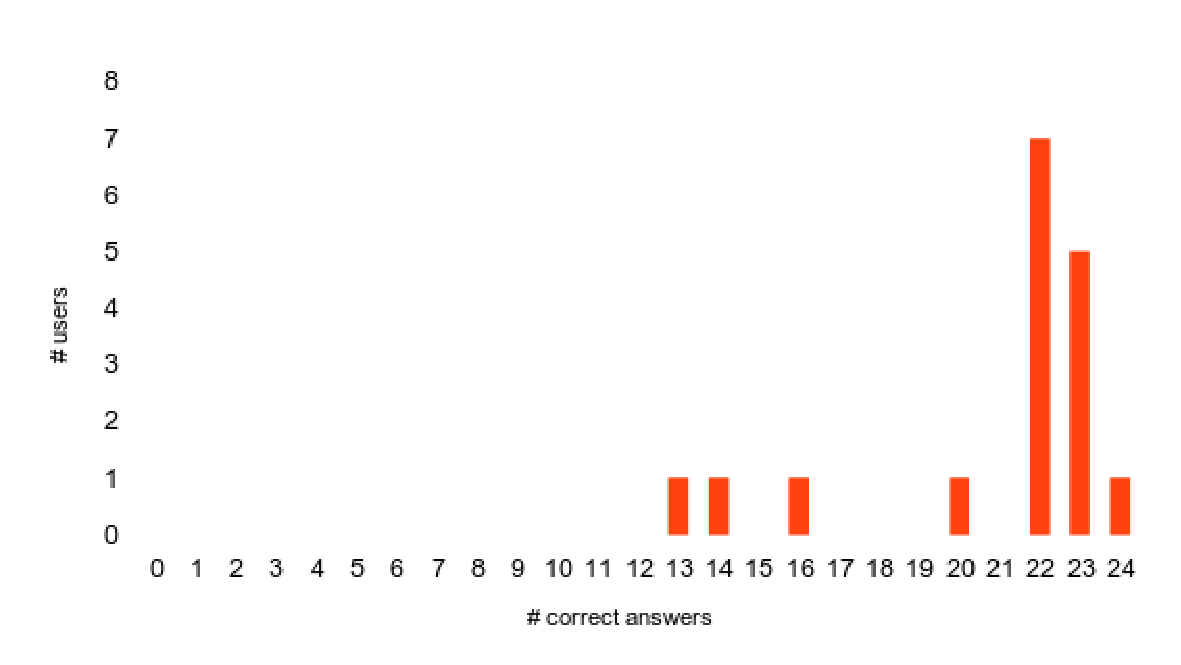
\includegraphics[width=0.45\textwidth]{hyp1a.pdf}}
\subfigure[After (New URLs Only)]{\label{fig:hyp1resultsanew}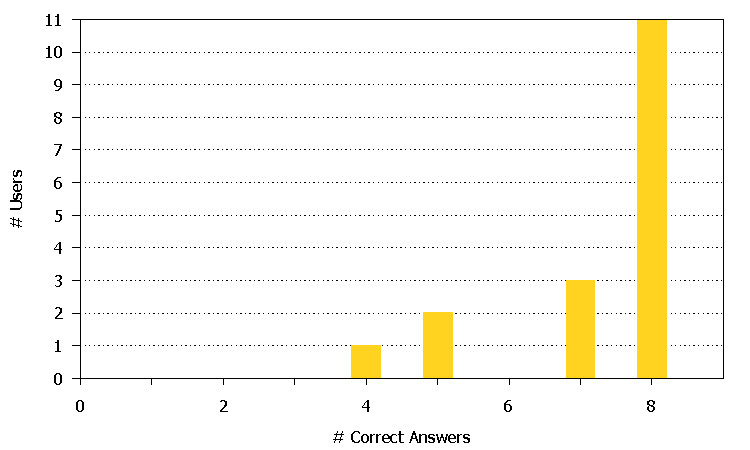
\includegraphics[width=0.45\textwidth]{hyp1anew.pdf}}
\subfigure[After (Repeated URLs Only)]{\label{fig:hyp1resultsarepeat}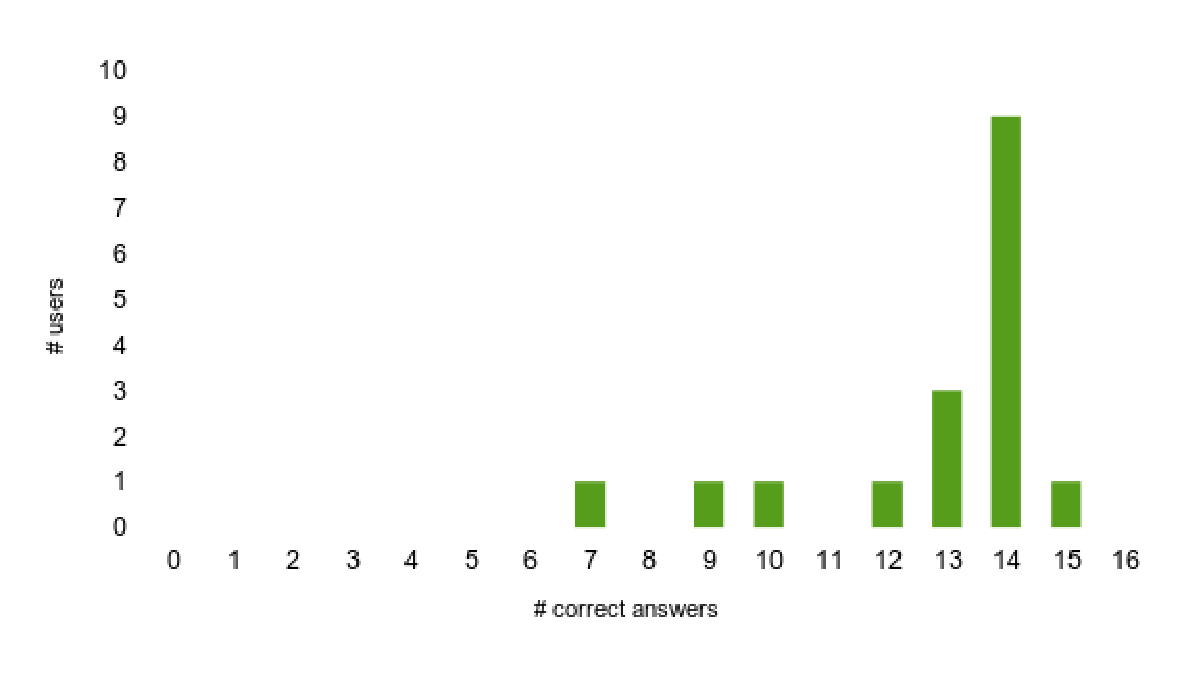
\includegraphics[width=0.45\textwidth]{hyp1arepeat.pdf}}
\caption{Correct Answers}
\label{fig:hyp1results}
\end{figure}

\begin{figure}
\centering
\subfigure[Before]{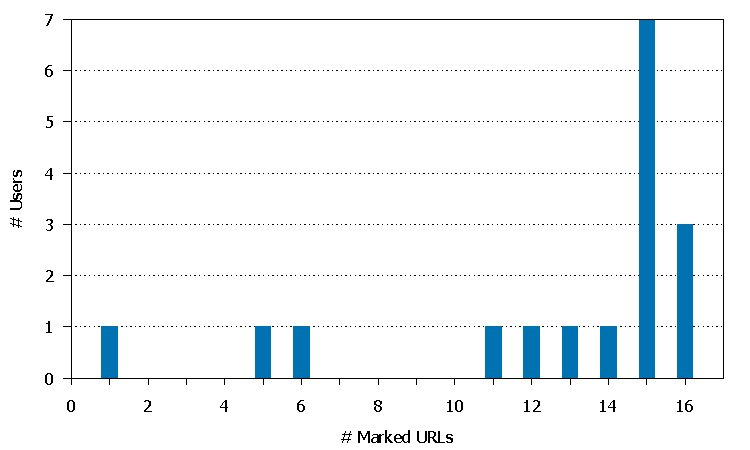
\includegraphics[width=0.45\textwidth]{hyp2b.pdf}}
\subfigure[After]{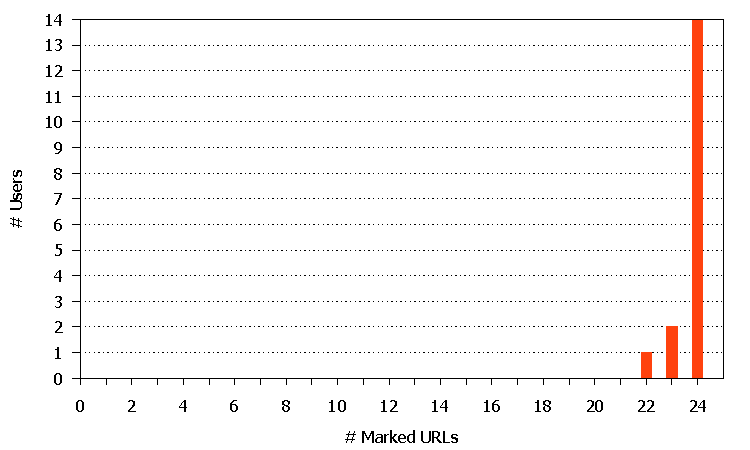
\includegraphics[width=0.45\textwidth]{hyp2a.pdf}}
\caption{URL marked}
\label{fig:hyp2results}
\end{figure}

\begin{figure}
\centering
\subfigure[Before]{\label{fig:domain_before}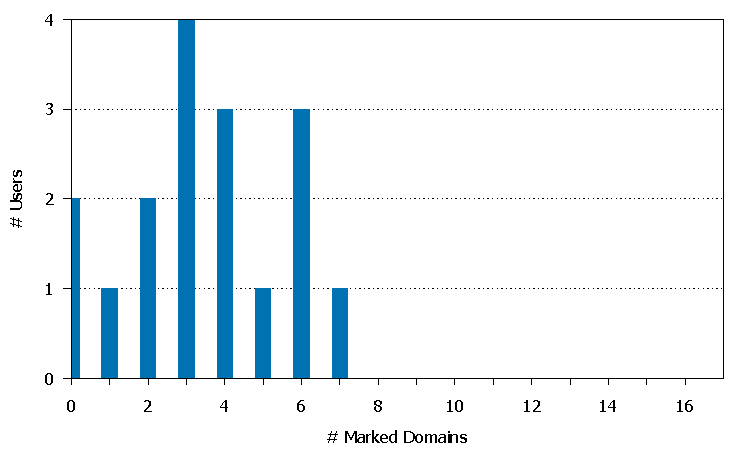
\includegraphics[width=0.45\textwidth]{hyp3b.pdf}}
\subfigure[After]{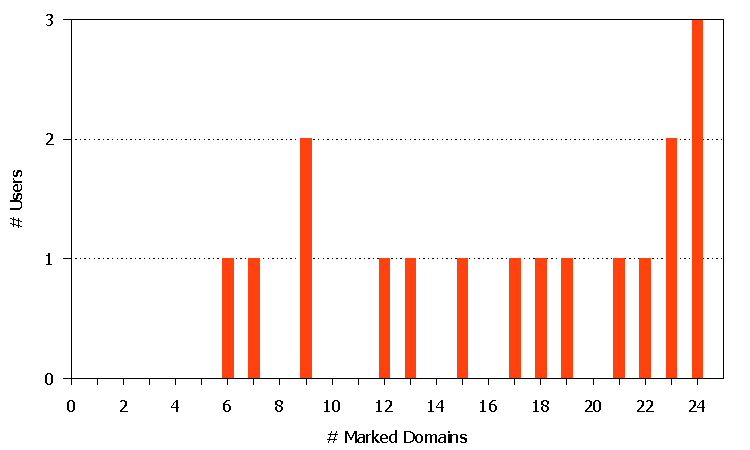
\includegraphics[width=0.45\textwidth]{hyp3a.pdf}}
\caption{Domain marked}
\label{fig:hyp3results}
\end{figure}

\begin{description}[leftmargin=0cm]
\item[Hypothesis 1:]
\autoref{fig:hyp1results} shows the results of our study according to hypothesis 1. One can clearly see that the majority of the users identified more URLs correctly after using the app than before. While most participants correctly identified 8 out of 16 (50\%) websites before they played the app, almost everyone gave correct answers to at least 22 out of 24 websites afterwards (cf. \autoref{fig:hyp1resultsbefore} and \autoref{fig:hyp1resultsaall}). One could argue that this increase is based on the fact that the examples are mainly the same in the website-survey after, i.e. the reason for their better performance is based on learning effects. \autoref{fig:hyp1resultsanew} however shows that the users also performed well for the new URLs. Therefore, we assume the learning effects are negligible.
In order to affirm our hypothesis we decided to apply the onesided Wilcoxon signed-rank test~\cite{wilcoxon1945individual} with our 16 samples from the website-survey before and the same 16 samples from the website-survey after.
Since we consider the learning effects negligible, we do not apply an alternative test against the 24 after URLs.
Our null hypothesis is $H_{0}: x_{1} >= x_{2}$ and the alternative hypothesis $H_{1}: x_{1} < x_{2}$, where x$_{1}$ represents the number of URLs which were correctly answered before playing the app and x$_{2}$ represents the number of URLs which were correctly identified after playing the app.
We computed the positive and negative rank-sums of $W_{+} = 141.5$ and $W_{-} = 11.5$.
The test statistic $w$ is the minimum of $W_{+}$ and $W_{-}$, hence $w = 11.5$.
As we chose $\alpha = 5\%$ as significance level and had 17 participants this results in a critical value of $41$.
As our test value $w = 11.5 < 41$ the null hypothesis can be rejected and thus the alternative $H_{1}$ is accepted.
Consequently, after playing the app the participants gave more correct answers than before.
We are confident that these results cannot entirely be reduced to learning effects.
Therefore, we believe that our app helped users to make improved decisions about the legitimacy of URLs.
\item[Hypothesis 2:]
\autoref{fig:hyp2results} shows how many users marked the URL as their main source of decision.
Most of the users already based most of their decisions on the URL before.
Occasionally users marked the content or the padlock (37 markings).
Afterwards, only 1 content was marked.
However, only 3 users (17.65\%) always marked the URL.
Afterwards, 14 users (82.35\%) always based their decision on the URL and only 3 users made one or two mistakes.
Therefore, we believe that our app emphasized their belief in basing their decision on the URL.
We decided against applying a statistical test to this hypothesis since there is obviously no signficant difference before and after playing the app.
\item[Hypothesis 3:]
There is a general problem with one question in the websites-surveys.
In the website-before survey we were not able to clearly ask the user to mark the domain when it was the base of his decision because we would have then primed them towards looking at the URL or even at the domain.
This would have influenced the results of hypothesis 2.
Since we could not formulate this question clearly, a user might have marked the whole URL even if his decision was based only on a small part (for example, the domain) of the URL.
Consequently, we were not able to clearly identify what the users' main source of decision was in the website-before survey.
We were aware of this problem beforehand but saw no other option than formulating the question in such an open form.
Afterwards, the user knew that they were expected to mark the domain.
This can be interpreted as a change of question even if the literal question did not change.
Therefore, we cannot apply any statistical tests on this hypothesis.
Yet, we want to have a look at the results.
None of the users marked the domain in most cases beforehand, in particular, 7 domains out of 16 URLs where marked at most by only one user, cf. \autoref{fig:domain_before}.
\begin{figure}
\centering
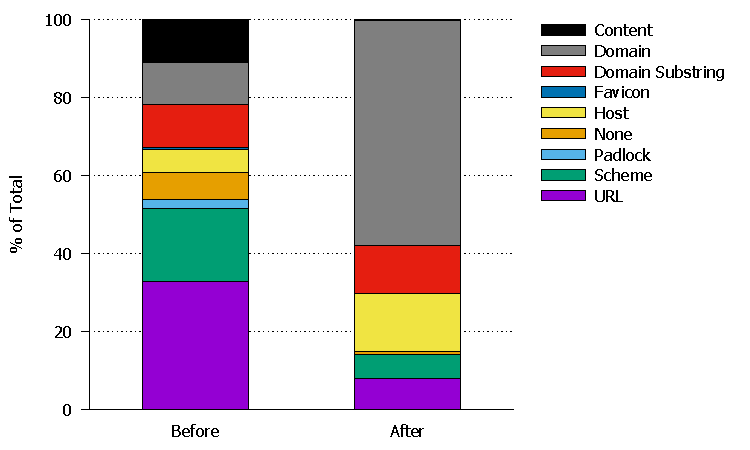
\includegraphics[width=0.65\textwidth]{markings.pdf}
\caption{Marked parts of the screenshot before and after}
\label{fig:markings}
\end{figure}

\begin{figure}
\centering
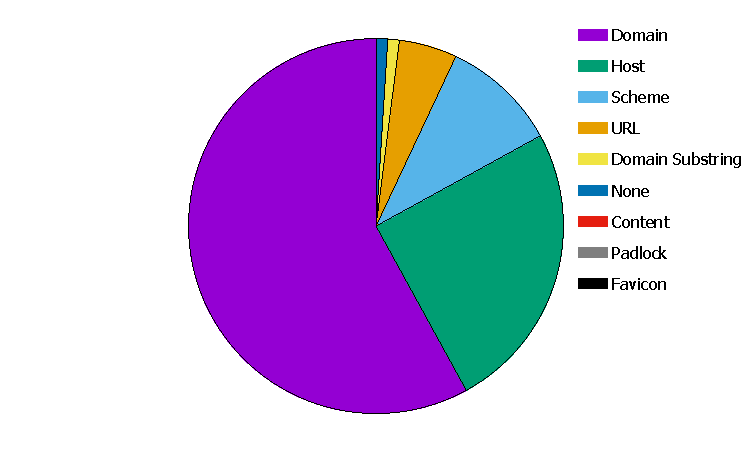
\includegraphics[width=0.65\textwidth]{legitimate_markings_after.pdf}
\caption{Marked URL parts of legitimate URLs}
\label{fig:legitimate_markings_after}
\end{figure}
\autoref{fig:markings} shows the distribution of the marked areas before and after playing our app. Obviously, afterwards most of the users marked the domain. However we are not able to compare that to the before values because of the changed question.
Another interesting observation is that quite a number of participants marked the complete host (instead of the domain) in case of legitimate URLs, cf.~\autoref{fig:legitimate_markings_after}. One explanation for this might be that we did not ask the user to mark the domain of legitimate URLs except in level 1.
\item[Hypothesis 4:]
According to the answers that the users gave in the After survey SUS section (\autoref{s:after_survey}) we calculated a SUS of 83.1. This is above 68 which means that we can consider our app above average usable.
\end{description}

%.........................................................................................................
\subsubsection{Further Study Outcomes}
%.........................................................................................................
\label{s:further_exploration}
Besides the results of our hypotheses the study yielded some further interesting outcomes.
This section further explores the results we obtained from our survey data and where not part of our hypotheses.
Afterwards, we summarize the participants' remarks to our app.

%.........................................................................................................
\paragraph{Further Data Exploration}
\begin{description}[leftmargin=0cm]
	\item[Correct and Reasoned Answers:] Hypothesis 1 only refers to giving a correct answer to the question whether a website is a phish or not.
	Our results show that users did not only give more correct answers after playing the app.
	In addition to their correct answer they reasoned their answer appropriately (i.e. marked the domain).
	In the website-survey before 37.5\% of the URLs were answered and reasoned correctly.
	After playing the app 75\% of the URLs were correctly identified and reasoned. 
	Note, that reasoned means by our definition that the domain was marked in addition to giving a correct answer.
	However, a reasoning must not always rely on the domain itself. 
	As discussed in \autoref{s:hypanalysis}, for example, there were numerous participants who often marked the host of legitimate URLs.
	This is a correct reasoning for their decision, however by our definition it was not considered as such.
	Also, there were plenty of users who detected a phish and marked the attacked part instead (cf. \autoref{fig:m_attack_recognized}).
	By our definition this was also not accepted as correct reasoning.
	Hence, if we had expanded our definition of reasoning even more users would have correctly reasoned their decisions.
	However, there is the question whether expanding the accepted answers might also result in an increase of the correct answers and markings in the before survey.
	\item[False Negatives and Positives:] Additionally we considered separately whether the user falsely  accepted phishes or rejected legitimate websites. Our outcomes show that before in average the user rejected 4.9 legitimate websites and accepted 2.1 phishing websites.
	After using the app the user rejected 1.8 legitimate websites and accepted 1.3 phishing websites.
	One must however note that we increased the users' attention by telling them to look for phishing websites.
	This means that they actively searched for traps and looked for reasons why they should not enter their data.
	In reality however the users contrarily have an interest in entering their personal data otherwise they would have not opened the website.
	Additionally, usually users tend to behave oversafely in lab situations \cite{wu2006security, egelman2007security}.
	Therefore we assume that in this situation, especially before playing the app, users tended to reject URLs in general for safety's sake.
	This is also reflected by the high rate of falsely rejected legitimate URLs.
	Nevertheless the results show that the users make less mistakes after playing the app and seem to better know why they reject or accept websites (cf. \autoref{s:hypanalysis}).
	In future this should be tested in a more realistic scenario where the users' attention is less increased towards looking for phishes and the users are not in lab situations.
	\item[User Opinions to App:] A part of our surveys aspired to understand the users' opinions to our app.
	Section 3 of our general-survey after (cf.~\autoref{s:after_survey}) contains the statements which the users had to assess with the aid of a 5 point Likert scale.
	Our worst, but still decent, score referred to whether the user was motivated by the spoofed e-mail to continue playing the app (median of 4) and whether the amount of texts was appropriate (median of 4).
	All other statements were strongly agreed (median of 5) with in median.
	The text legibility of our app texts received a median score of 5.
	Our study participants strongly agreed (median of 5) that our app helped them to identify phishing websites in the future.
	Finally, the users intuitively understood our three lives scheme per level (median of 5).
	Thus, the outcomes of the user opinions reveal that our app was very well received by the participants regarding these questions.
	\item[Achieved Levels:] In average the participants reached level 7, which is higher than we had expected.
	We assume that some users started to roughly scan our texts for relevant information (for example, mainly looking at the examples) after they understood the importance of the domain.
	One user even played through the app in 30 minutes.
	In fact, this user has performed worse by the terms of our definition of correctness.
	The user had correctly identified 9 (75\%) of the URLs before playing the app.
	Afterwards, he only had a score of 13 (54.17\%).
	The problem was that level 9 deals with the difference of HTTP and HTTPS websites.
	Pretests had shown that most users would not get beyond level 6. Therefore, we had not considered level 9 in our assessment strategy and regarding its impact on the question.
	Users were expected to decide whether a website is a phish or not disregarding the usage of HTTPS.
	The user who has achieved level 9 however was explained the difference of HTTP and HTTPS, additionally, he was asked to reject HTTP sites in general for this level.
	Hence, this user responded to the website-survey after respectively: the participant generally rejected HTTP sites whether they were phishing or not and thus the user performed worse afterwards by the terms of our definition of correct.
	All other users performed better after playing the app.
	\item[Relation Between Achieved Level and Identified Websites] 
		\begin{figure}
			\centering
			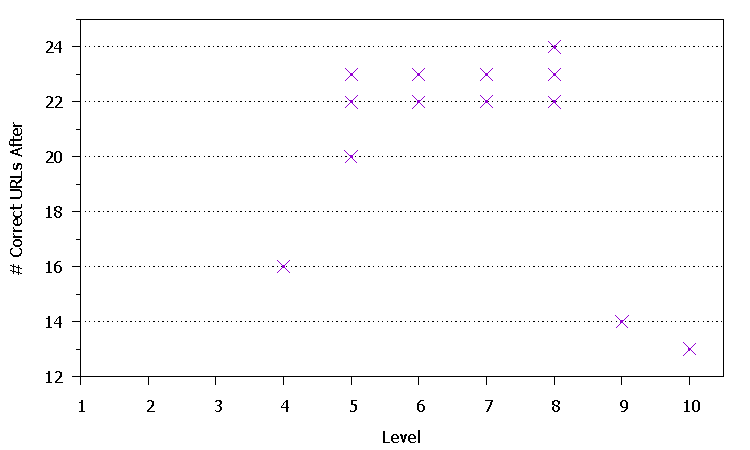
\includegraphics[width=0.85\textwidth]{correct_per_level.pdf}
			\caption{Correct answers related to achieved level}
			\label{fig:correct_per_level}
			\end{figure}
	\autoref{fig:correct_per_level} shows the relation between the levels a user achieved and his performance after playing the app. The performance decline of the users that played level 9 or even 10 is explained in the previous paragraph. These examples are not considered in the following. The Figure shows that playing level 5 already helped users to correctly identify URLs.
As we cannot ensure that all users will play our app through, we think it is good that the first levels already provide them the most important input which helps them make more correct decisions on the legitimacy of URLs. 
Nevertheless, we are confident that the succeeding levels help users detect more advanced attacks and thus are important. There are examples of users that fell for attacks in the website-survey after which they were not confronted with during the game.

We found 3 of these examples:
\begin{enumerate}
\item One participant who achieved level 5 in the game fell for an attack that was introduced in level 6 (paypal-sicher.de).
\item 11 participants fell for a phish with scrambled letters (mircosoft.com) which was introduced in level 6. These included users who achieved level 6 or higher as well as those who did not achieve this level. In the contrary, those participants who did not fall for this phishing URL at least achieved level 6, i.e. nobody of the users who did not play level 6 recognized this attack. 
\item 4 participants fell for an attack which was introduced in level 8. Three of these participants did not play level 8.
\end{enumerate}
	Note that all of the services presented by the URLs were known to the users, i.e. it is likely that they fell for the actual attack and did not just assume that the URLs might be legitimate.
	These aspects indicate that the later levels and training are important to achieve higher expertise.
	Due to the small sample size, with at most 1-2 examples per attack, it is possible that the above mentioned examples were slightly suppressed in \autoref{fig:correct_per_level}.
	An examination of the relation between the achieved level and the recognized attacks could be done in further research with a larger data set.
	\item[HTTPS and Padlock:] Our results show that some participants were aware that they should look for either HTTPS or a padlock before playing our app~\autoref{fig:markings}.
	For instance, one participant marked the scheme or the padlock as reason for his decision 11 out of 16 times in the website-survey before. 
	Another participant marked the scheme or the padlock of 8 examples.
	These participants trusted the padlock resp. HTTPS websites and distrusted HTTP.
	Consequently, they fell for phishing websites which make use of HTTPS in our survey and are likely to fall for such attacks in reality.
	Thus, the users who based their decisions on these indicators did not seem to be aware of the fact that the use of HTTPS does not necessarily mean that the website is trustworthy in general.
	In fact, there are phishing websites using HTTPS (cf. \autoref{fig:https_phish}). 
	Since we cannot assure that an app user of ours plays until level 9, we believe it is important to introduce the level dealing with HTTPS earlier.
	This aspect should definitely be considered in future work in our opinion.
	\item[User Self-Assessment:] Contrary to our expectations, users assessed themselves rather correctly. When asked for their ability of distinguishing legitimate from fraudulent websites at the beginning of the study they rated themselves with 3 on a 5 point Likert scale.
Their actual performace in the website-survey before is likewise (56\% correctly identified URLs). After using the app they were asked whether the app helped them identify phishing websites in the future. They rated 5 out of 5 and their performance was accordingly good (87\% correctly identifies URLs).
	\item[Confidence:] We asked the users how confident they were about their answers on the website-surveys on a 5 point Likert scale. In median before using the app 3 users stated a confidence of 5. Afterwards, there were 11 users that stated 5 in median. \autoref{fig:confidence} visualizes the overall increase of the users' confidence.
	\begin{figure}
		\centering
		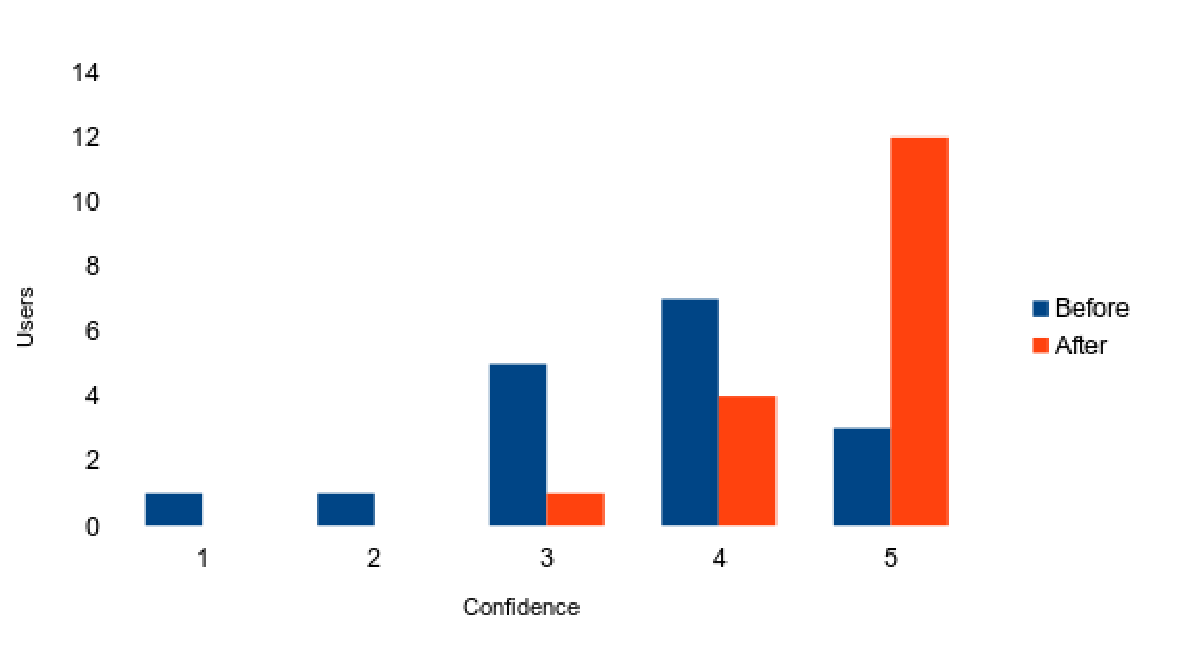
\includegraphics[width=0.85\textwidth]{confidence.pdf}
		\caption{Confidence of the users before and after}
		\label{fig:confidence}
		\end{figure}
\end{description}
\begin{figure}
	\centering
	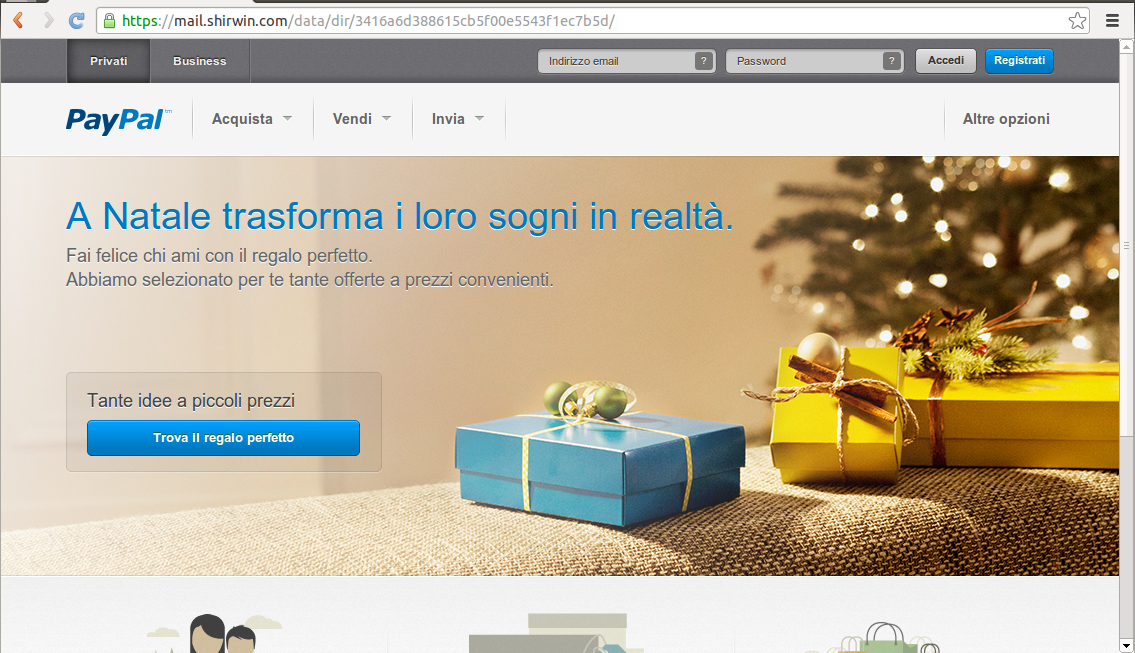
\includegraphics[width=0.9\textwidth]{https_phish.png}
	\caption{Phishing website using HTTPS~\cite{phishtank}}
	\label{fig:https_phish}
	\end{figure}
	
%.........................................................................................................
\paragraph{Remarks of Participants}
\label{s:remarks_of_participants}
During playing the app, the participants had a slip of paper for notes they wanted to make considering the app.
In the following we outline the main results of these slips of paper.
Note that we did not ask the users to write down something specific. 
We merely asked them to write down what they thought, i.e. there might be more participants who agreed with some of these points below but just have not explicitly written it down.
In the following we consider the notes and suggestions of all participants. 
\begin{description}[leftmargin=0cm]	
	\item[Scrolling of URL:] In addition to deciding whether a URL is a phish or not, the user has to face two more challenges. 
First, the font size gets increasingly smaller in higher levels, until it eventually is approximately the same size of the Android standard browser.
Second, the URL is displayed in a horizontal scrollbar so that the has to scroll the URL to the right in order to view the beginning of it, just like it is the case in browsers.
4 participants found this disturbing and said it hindered them from analyzing the URL reasonably. 
This supports the importance of the introduction part 2 (access address bar) in the app.
The scrolling is present in order to simulate the behavior in the browser and it is important for a user to practice this.
We assume that the users would not have noted this in this extent in case they had completed introduction part 2, because then they probably would have understood why we do the URL scrolling during the exercises.
Yet, we think after a couple of levels the users should have understood that they have to scroll the URL, in the game as well as in the browser, so one might consider to reduce or eliminate it after some time. 
	\item[Unknown Services:] We have mentioned the problem of unknown services in \autoref{s:problems_with_URLs}.
As we were afraid there are in fact services which are not familiar to several users.
Several participants mentioned this problem.
Even if we tried to make use of the most popular services with the aid of Alexa's~\cite{alexa} ranking we cannot assure that all used URLs are known by all users.
One idea to approach this challenge might be to provide an question mark button in addition to the check mark (no phish) and cross mark (phish) buttons. 
When a player clicks on this button, he can be told whether the given URL is a phish or not and why.
From this action the user would neither profit nor would he lose any points or lives.
Yet, we do not think that this is a major issue, since the users got at least until level 4 and most of them achieved even higher levels.
We are confident that the app in its current state is already implicitly able to teach the users about the legitimacy of unknown services.
After facing unfamiliar URLs and making or not making mistakes they will eventually learn whether to trust a service or not.
	\item[Question to Data Entry:] Some participants noted that the formulation of our website-survey question ``Would you enter your sensitive data into this website?'' was ambiguous.
Thus, there might have been participants who selected ``no'' even if they did not think it was a phishing website, but they would generally not enter their data into this specific website.
Originally, the website-surveys before and after asked the participants whether they thought a given website screenshot was a phishing website or not.
After our test iteration of our study, however, we decided to add some context to the question and had to make this trade-off with respect to the new question's ambiguity.
As we told the user that this study was particularly about phishing and that their task was to detect phishing websites in the website-surveys before and after, we believed that the ambiguity of this question would be negligible.
	\item[Explanations and Comprehensibility:]
4 participants stated on their slips of paper that they found the explanations of the app very good and easy to understand.
1 of these 4 participants, however, added that there is partially much text to read.
Another participant (not under those 4) noted that there is too much and long text in general.
	\item[Button Positioning:] The positioning of our app buttons during the game are as follows: 
The left bottom corner has a check mark which represents that the user thinks the displayed URL is not a phish.
The right bottom corner has a cross mark which means that the user thinks the displayed URL is a phish.
After clicking on either of these buttons in the write bottom corner another button appears (where the cross mark usually is) which either is the continue or the verify button (depending on whether the user has to select the Who-Section or not).
Some participants indicated that the positioning of the buttons in the right bottom corner are suboptimal.
The problem is that accidentally double clicking, for example, the continue button in the right corner results in rejecting the next URL even if the user might not have intended to.
Even if not many participants explicitly criticized this aspect we believe that this is a justified point.
In fact, the positioning of the two buttons continue and verify should be different from the one of the cross mark.
This is an aspect which should be targeted in future work. 
	\item[Repetition:]
Repetition is an important element of our app.
In every level introduction we briefly repeat the so far learned parts of a URL (with a graphic) and the different attacks the user has seen until this point.
We also make use of repetitions during the exercise rounds, every level contains at least one exercise from the previous level.
Some of our participants explicitly indicated that our repetitions made them feel more confident and safer.
	\item[External Links:]
In the main menu of our app we have a button ``More About Phishing'' which leads to a list of external links to various websites about phishing.
Some of these websites are in English.
Some participants indicated that they did not like it to be led to an English website and would have preferred to be forwarded to a German one.
This reveals that we cannot expect our audience to have knowledge of the English language.
Therefore, only German websites should be linked in the future.
Another idea to approach this might be to provide in-app additional information.
That is, instead of linking to external websites, the app itself could provide additional categorized information in German.
This would solve the problem with the language of websites and at the same time the additional information would fit to our app layout and design.
	\item[Amount of Examples:] Our app starts with a small sample of URLs users have to decide on.
In every level the sample size increases as the number of possible attacks increases.
Only 2 participants found that our sample size was too large.
This might have been the result of the fact that the users had to play the game for half an hour at a time.
We believe that the number of examples are reasonable, assumed that a user does finish the app at a stroke.
	\item[Further Suggestions:] In their notes some users made several suggestions which we found interesting.
These suggestions include, for example, more text highlighting of new teaching contents or the suitability of our app to be applied in schools.
In \autoref{s:future_work} we elaborate on aspects for further research in more detail.
\end{description}

\subsection{Limitations}
We decided to conduct a study which compares the users' performance before and after playing our educational app.
Our study design has some limitations we were not able to address for several reasons that we are going to discuss subsequently.

\begin{description}[leftmargin=0cm]
	\item[Behavior Change:] In our study the participants were not in their usual environment. 
	Therefore, they likely behaved differently during our study.
	An alternative approach would have been to distribute the app to several participants and ask them to play it remotely.
	However, this has two major downsides: First, the user would have been remote and thus we would have less control.
	Second, testing the before and after app skills would have been difficult to realize in order to ensure a homogenous process among all participants.
	\item[Increased Attention:] At the beginning of the study the participants were told that the study dealt with phishing.
	Additionally, for the website-survey before and after they were explicitly asked to indicate whether the websites were phishing or not.
	That is to say, the user automatically increased his attention towards answering these kinds of questions.
	Designing an in situ study, where the participant would have been in their usual environment and would have not known about their participation, was not considered because such a design is ethically and legally questionable. 
	\item[Knowledge Retention:] Our study design focuses on the present.
	Given certain time boundaries, it was not possible to study the long-term influences of our app by conducting the after app scenario repeatedly. 
	Consequently, knowledge retention is an aspect which is not considered by our study.
	\item[Bias:] For the recruitment we endeavored to ensure that our participants are not close friends of ours. 
	We rather seeked for friends of friends or even completely unknown persons~(cf. \autoref{s:participant_recruitment}).
	Certainly, the presence of a minor bias cannot be totally excluded.
\end{description}
Despite the limitations of our study we are confident that we got a good insight into the effectiveness of our app.

%===========================================
\subsection{Discussion}
%===========================================
Our hypotheses stated that our app can increase three major skills of the user.
First, we wanted to give the user the ability to detect phishing URLs.
This goal can be considered achieved as we could show that the increase is significant.
Even though there might be some learning effect we are confident that this increase is not mainly attributable to that.
The second and third hypotheses focused on the reasoning behind the user's decision.
We wanted to show that the user is aware of the fact that the content is no source of evidence against a phishing attack.
Our results suggest that most of the users already feel that the URL is important beforehand but some additionally consider the content.
Thus, the change in user response was not high enough to measure our hypothesis 2. 
The third hypothesis said that the users understand the structure of URLs better after playing our app.
As we discussed above, we had concerns about the design of the question that was intended to test this hypothesis.
The question has to be regarded as changed after playing the app.
Due to this, we could not consider the before-markings and could not argue on any findings about this hypothesis.

In addition to testing the hypotheses we got overall positive feedback from the users.
Most of them had the feeling they learned something from the app.
Some participants even contacted us asking about the release date of the app because they wanted to give it to their relatives.

Yet, there are still some improvements that should be considered when someone develops a next version of the app.
First of all, we think that the part talking about HTTP and HTTPS should be moved to an earlier level.
We saw many users that marked the scheme or the padlock in the URLs in the website-survey before.
This seems to be more important for the user than the URL itself because we had several users who fell for a phish and marked the scheme or padlock as reasoning.
As we cannot assume that users finish our app within one day, or even finish it at all, we think that it is important to clear that misunderstanding earlier.
The second improvement that a following developer should include is to restructure the app texts in such a way that the user can clearly identify repeating and new parts.
We think this aspect is not as important in real life compared to study situations because the app is not designed to be played a long time in a row.
This would increase the importance of the repetitions and make such a separation less important but this can be improved.
Last, it might be a good improvement to modify the app behavior depending on the user skill and performance.
This might prevent the user from getting bored.
This includes, for instance, vary feedback texts and icons depending on the user's performance as well as the degree of difficulty.
Another example is that the app could skip the proof part (identify Who-Section after detection of a phish) in case there is an indication that the user understood how to do it.
A simple form of that is already implemented.
The proof is shown up to a predefined level.
Yet, we think it is more reasonable to base the skipping and other possible extensions on the user performance. 

To conclude our findings despite some possibilities for improvement we can say that the app helped most of the users detect phishing URLs. This means we overall achieved the goal of the app.
